\section{Experimental Setup}

We design experiments to answer three research questions:

\textbf{RQ1:} Is the 134-problem EvalPlus failure set fully recoverable from archive for
reproducible repair experiments?

\textbf{RQ2 (Pre-registered):} Does specification-aligned repair (Condition C) achieve
significantly higher round-1 pass@1 than blind reprompting (Condition B)?

\textbf{RQ3 (Pre-registered, Exploratory):} Does the HumanEval$+$ fix rate exceed MBPP$+$
under Condition C?

\subsection{Dataset}

\begin{table}[h]
\centering
\caption{EvalPlus failure set composition.}
\label{tab:dataset}
\begin{tabular}{lcc}
\toprule
Benchmark & Failures & \% of total \\
\midrule
HumanEval$+$ & 34 & 25.4\% \\
MBPP$+$ & 100 & 74.6\% \\
\textbf{Total} & \textbf{134} & \textbf{100\%} \\
\bottomrule
\end{tabular}
\end{table}

\begin{figure}[t]
\centering
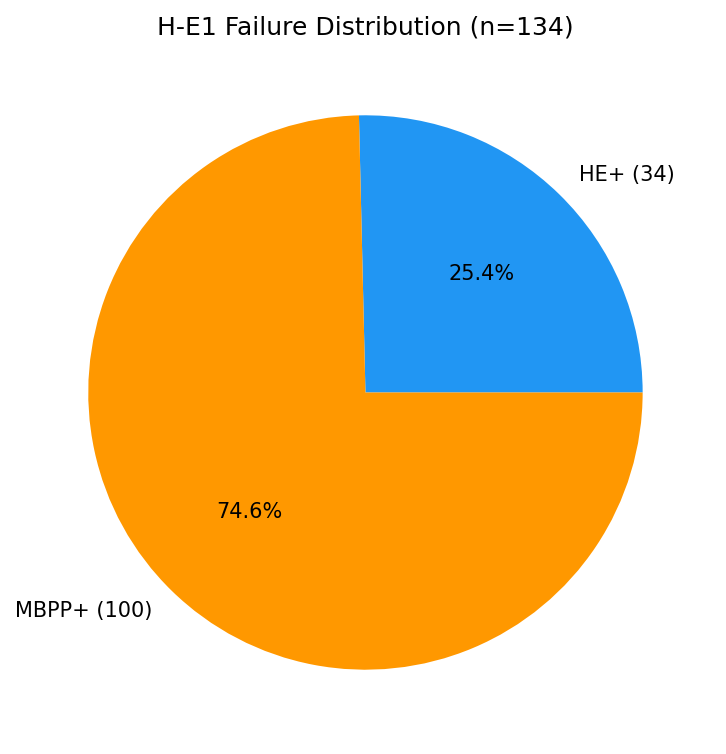
\includegraphics[width=0.7\textwidth]{figures/failure_distribution.png}
\caption{Distribution of GPT-4o-mini round-0 failures on EvalPlus: 34 HumanEval$+$ (25\%) and 100 MBPP$+$ (75\%) problems, totaling 134 failures that define the working set for specification-aligned repair experiments.}
\label{fig:failure-distribution}
\end{figure}

Figure~\ref{fig:failure-distribution} shows the failure distribution. All 134 failures are semantic/algorithmic
errors: ruff$+$mypy fire on at most 32.4\% of HumanEval$+$ and 16.0\% of MBPP$+$ failures.

\textbf{Working set.} 128 tasks (6 excluded for empty \texttt{plus\_fail\_tests}; 95.5\% recovery).

\begin{figure}[t]
\centering
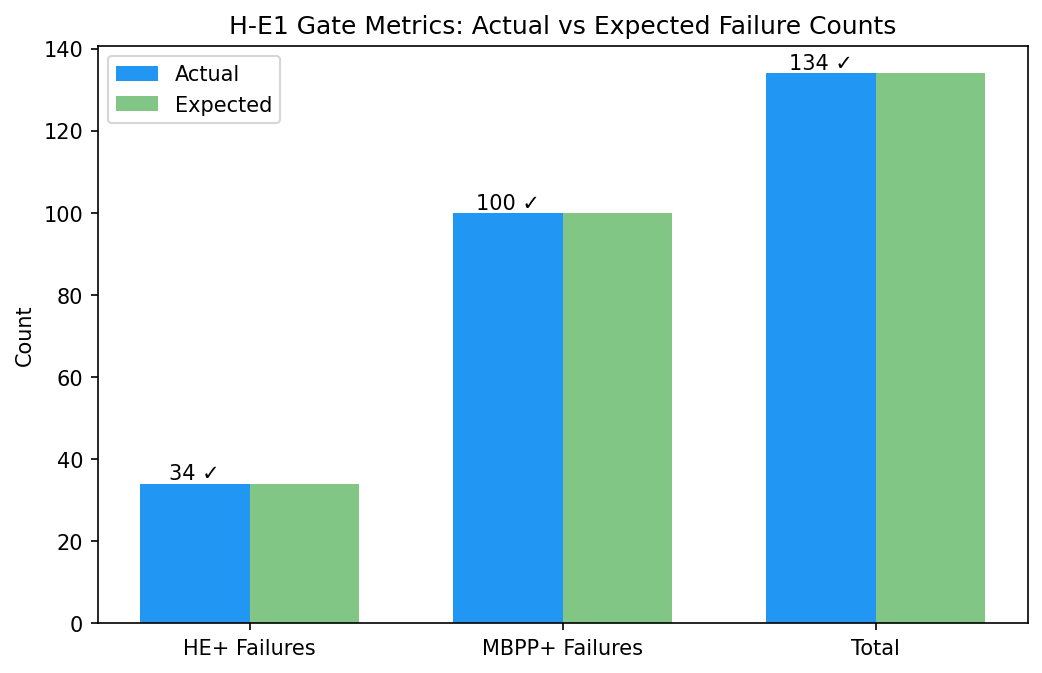
\includegraphics[width=0.7\textwidth]{figures/gate_metrics.png}
\caption{Actual vs. expected failure counts from the h-e1 Run 2 archive, confirming 34 HumanEval$+$ and 100 MBPP$+$ failures match pre-registered targets.}
\label{fig:gate-metrics}
\end{figure}

\subsection{Baselines}

\begin{table}[h]
\centering
\caption{Experimental conditions and rationale.}
\label{tab:baselines}
\begin{tabular}{lll}
\toprule
Condition & Method & Rationale \\
\midrule
A & h-e1 Run 2 results & Failure population ground truth \\
B & Fixed reprompt (\citealt{Madaan2023} motivation) & Placebo control: re-exposure without error context \\
C & This work (specification triple) & Tests semantic gap description oracle \\
\bottomrule
\end{tabular}
\end{table}

\subsection{Evaluation Metrics}

\textbf{Primary:} Round-1 pass@1 --- binary fix per problem; code must pass \textit{all} EvalPlus
augmented tests (not just the prompted failing test).

\textbf{Secondary:} Fix rate (proportion fixed; Condition C threshold $\geq$ 15\%), token
efficiency ratio (fix rate per 1000 additional input tokens vs. Condition A).

\subsection{Implementation Details}

\begin{itemize}
\item Model: GPT-4o-mini (OpenAI API), temperature$=$0.2, seed$=$42
\item Test selection: \texttt{plus\_input[0]} (deterministic, pre-registered)
\item Evaluation oracle: EvalPlus augmented test suite (all tests must pass)
\item EvalPlus version: 0.3.1
\item Estimated mechanism experiment cost: $\sim$\$0.05 (256 API calls total)
\end{itemize}
